%Version 3.1 December 2024
% See section 11 of the User Manual for version history
%
%%%%%%%%%%%%%%%%%%%%%%%%%%%%%%%%%%%%%%%%%%%%%%%%%%%%%%%%%%%%%%%%%%%%%%
%%                                                                 %%
%% Please do not use \input{...} to include other tex files.       %%
%% Submit your LaTeX manuscript as one .tex document.              %%
%%                                                                 %%
%% All additional figures and files should be attached             %%
%% separately and not embedded in the \TeX\ document itself.       %%
%%                                                                 %%
%%%%%%%%%%%%%%%%%%%%%%%%%%%%%%%%%%%%%%%%%%%%%%%%%%%%%%%%%%%%%%%%%%%%%

% \documentclass[referee,sn-basic,Numbered]{sn-jnl}% referee option is meant for double line spacing


%%=========================================================================================%%
%% the documentclass is set to pdflatex as default. You can delete it if not appropriate.  %%
%%=========================================================================================%%

%%\documentclass[sn-basic]{sn-jnl}% Basic Springer Nature Reference Style/Chemistry Reference Style

%%Note: the following reference styles support Namedate and Numbered referencing. By default the style follows the most common style. To switch between the options you can add or remove �Numbered� in the optional parenthesis. 
%%The option is available for: sn-basic.bst, sn-chicago.bst%  
 
%%\documentclass[pdflatex,sn-nature]{sn-jnl}% Style for submissions to Nature Portfolio journals
%%\documentclass[pdflatex,sn-basic]{sn-jnl}% Basic Springer Nature Reference Style/Chemistry Reference Style
\documentclass[pdflatex,sn-mathphys-num]{sn-jnl}% Math and Physical Sciences Numbered Reference Style
%%\documentclass[pdflatex,sn-mathphys-ay]{sn-jnl}% Math and Physical Sciences Author Year Reference Style
%%\documentclass[pdflatex,sn-aps]{sn-jnl}% American Physical Society (APS) Reference Style
%%\documentclass[pdflatex,sn-vancouver-num]{sn-jnl}% Vancouver Numbered Reference Style
%%\documentclass[pdflatex,sn-vancouver-ay]{sn-jnl}% Vancouver Author Year Reference Style
%%\documentclass[pdflatex,sn-apa]{sn-jnl}% APA Reference Style
%%\documentclass[pdflatex,sn-chicago]{sn-jnl}% Chicago-based Humanities Reference Style

%%%% Standard Packages
%%<additional latex packages if required can be included here>

\usepackage{graphicx}%
\usepackage{multirow}%
\usepackage{amsmath,amssymb,amsfonts}%
\usepackage{amsthm}%
\usepackage{mathrsfs}%
\usepackage[title]{appendix}%
\usepackage{xcolor}%
\usepackage{textcomp}%
\usepackage{manyfoot}%
\usepackage{booktabs}%
\usepackage{algorithm}%
\usepackage{algorithmicx}%
\usepackage{algpseudocode}%
\usepackage{listings}%

%%%%

%%%%%=============================================================================%%%%
%%%%  Remarks: This template is provided to aid authors with the preparation
%%%%  of original research articles intended for submission to journals published 
%%%%  by Springer Nature. The guidance has been prepared in partnership with 
%%%%  production teams to conform to Springer Nature technical requirements. 
%%%%  Editorial and presentation requirements differ among journal portfolios and 
%%%%  research disciplines. You may find sections in this template are irrelevant 
%%%%  to your work and are empowered to omit any such section if allowed by the 
%%%%  journal you intend to submit to. The submission guidelines and policies 
%%%%  of the journal take precedence. A detailed User Manual is available in the 
%%%%  template package for technical guidance.
%%%%%=============================================================================%%%%

%% as per the requirement new theorem styles can be included as shown below
\theoremstyle{thmstyleone}%
\newtheorem{theorem}{Theorem}%  meant for continuous numbers
%%\newtheorem{theorem}{Theorem}[section]% meant for sectionwise numbers
%% optional argument [theorem] produces theorem numbering sequence instead of independent numbers for Proposition
\newtheorem{proposition}[theorem]{Proposition}% 
%%\newtheorem{proposition}{Proposition}% to get separate numbers for theorem and proposition etc.

\theoremstyle{thmstyletwo}%
\newtheorem{example}{Example}%
\newtheorem{remark}{Remark}%

\theoremstyle{thmstylethree}%
\newtheorem{definition}{Definition}%

\raggedbottom
%%\unnumbered% uncomment this for unnumbered level heads

\begin{document}

\title[Using Trie Data Structure for Efficient Database Index Representation]{Using Trie Data Structure for Efficient Database Index Representation}

%%=============================================================%%
%% GivenName	-> \fnm{Joergen W.}
%% Particle	-> \spfx{van der} -> surname prefix
%% FamilyName	-> \sur{Ploeg}
%% Suffix	-> \sfx{IV}
%% \author*[1,2]{\fnm{Joergen W.} \spfx{van der} \sur{Ploeg} 
%%  \sfx{IV}}\email{iauthor@gmail.com}
%%=============================================================%%

\author{\fnm{Maksym} \sur{Voroniy}}\email{maksym.voroniy.research@gmail.com}

%%==================================%%
%% Sample for unstructured abstract %%
%%==================================%%

\abstract{Modern database systems rely heavily on time-proven algorithms for
representing and organizing data on external storage. At the same time,
they must continuously adapt to evolving hardware architectures and
changing business demands - such as horizontal scalability for big data
workloads and the emergence of vector databases driven by the rapid
growth of AI applications.

A vast body of scientific and engineering work has focused on the
adaptation and optimization of well-known tree-based indexing structures
- such as B-trees, B\textsuperscript{+}-trees, B\textsuperscript{*}-trees, and R-trees - to meet these
challenges. These structures have become foundational to modern storage
engines due to their strong performance characteristics on
block-oriented storage systems.

This article, however, aims to draw attention to a different class of
data structures, referred to by Donald Knuth as digital searching
techniques \cite{knuthVol3}. Among these, the Trie (also known as a prefix tree)
occupies a special place. Unlike comparison-based trees, Tries organize
data according to the structure of keys themselves, making them
particularly well-suited for representing and indexing wide range of
digital data not only well known strings, but bit sequences, and encoded
numbers or even vectors.

This article serves as the first in a series exploring how Trie-based
data structures can be applied to address modern, complex indexing
problems. The goal is to demonstrate how Tries enable efficient,
scalable, and structurally expressive representations for arbitrary data
- offering alternative design trade-offs that are increasingly relevant
in contemporary database and data-intensive systems.
}

%%================================%%
%% Sample for structured abstract %%
%%================================%%

% \abstract{\textbf{Purpose:} The abstract serves both as a general introduction to the topic and as a brief, non-technical summary of the main results and their implications. The abstract must not include subheadings (unless expressly permitted in the journal's Instructions to Authors), equations or citations. As a guide the abstract should not exceed 200 words. Most journals do not set a hard limit however authors are advised to check the author instructions for the journal they are submitting to.
% 
% \textbf{Methods:} The abstract serves both as a general introduction to the topic and as a brief, non-technical summary of the main results and their implications. The abstract must not include subheadings (unless expressly permitted in the journal's Instructions to Authors), equations or citations. As a guide the abstract should not exceed 200 words. Most journals do not set a hard limit however authors are advised to check the author instructions for the journal they are submitting to.
% 
% \textbf{Results:} The abstract serves both as a general introduction to the topic and as a brief, non-technical summary of the main results and their implications. The abstract must not include subheadings (unless expressly permitted in the journal's Instructions to Authors), equations or citations. As a guide the abstract should not exceed 200 words. Most journals do not set a hard limit however authors are advised to check the author instructions for the journal they are submitting to.
% 
% \textbf{Conclusion:} The abstract serves both as a general introduction to the topic and as a brief, non-technical summary of the main results and their implications. The abstract must not include subheadings (unless expressly permitted in the journal's Instructions to Authors), equations or citations. As a guide the abstract should not exceed 200 words. Most journals do not set a hard limit however authors are advised to check the author instructions for the journal they are submitting to.}

\keywords{Trie, Prefix Tree, Database Indexing,
    Memory-Efficient Data Structures, Bitmap Indexing, Page-Oriented Storage}

%%\pacs[JEL Classification]{D8, H51}

%%\pacs[MSC Classification]{35A01, 65L10, 65L12, 65L20, 65L70}

\maketitle

\section{Introduction}\label{sec1}


Improving the efficiency of a data structure does not necessarily require replacing its fundamental algorithm. In many practical cases, the largest gains can be achieved by reconsidering how the existing structure is represented in memory.

Trie-based structures provide a particularly illustrative example. A straightforward Trie implementation can represent each node as a fixed-size lookup table indexed by the alphabet. Such a representation provides constant-time navigation, but its memory consumption is proportional to the size of the alphabet rather than to the actual number of children of a node. For sparsely populated nodes, the majority of the allocated space therefore represents absent edges.

A common approach to this problem is to introduce progressively more sophisticated node representations: hash tables, sorted arrays, or adaptive node types selected according to the number of stored children. These techniques improve the utilization of allocated memory, but they still leave an important question: what is the appropriate unit at which the optimization should be applied?

This work follows a different principle. Rather than making small, isolated modifications to the Trie algorithm, it treats the node representation itself as an optimization target. In particular, the proposed approach separates the identification of existing edges from their physical storage. A compact bit-indexed structure can represent the presence of children over the complete alphabet, while a contiguous array stores only the actually existing entries. This makes it possible to preserve constant-time navigation and ordered traversal while avoiding the space cost of empty lookup-table entries.

The objective is therefore not to propose a radically different indexing algorithm, but to demonstrate how small changes in the representation at the right structural level can produce substantial improvements in memory efficiency of the Trie. The following sections develop this idea from the basic Trie representation through sparse-node compression, bit-indexed navigation, and specialized root handling.


\section{Results}\label{sec2}

\begin{itemize}
\item Introduced a step-by-step approach to formalizing the Trie data structure as a foundation for further research.
\item Proposed a space-efficient node representation based on bitmap indexing and compact arrays for sparsely populated Trie nodes.
\end{itemize}

\section{Informal Trie introduction}\label{informal_intro}

A Trie, also known as a prefix tree or digital tree, is a tree-based data structure
originally developed for storing and efficiently retrieving strings. Unlike
comparison-based search trees, where a complete key is typically stored in a node
and compared with other keys, a Trie represents a key by a path from the root through a sequence of nodes.

The simplest - though informal - way to introduce the Trie data
structure is to start by grouping several strings and observing their
shared prefixes. Consider the following set of words:

\{car, cart, computer, cat\}

The common prefix for all words is "c". The words "car", "cart", and
"cat" additionally share the prefix "ca", while "car" itself is a common
prefix of "car" and "cart".

Figure~\ref{fig:3word} illustrates the corresponding prefix tree constructed from this
set of words.


\begin{figure}[h]
\centering

\includegraphics{images/media/01.3-word}
\caption{Simple prefix tree}\label{fig:3word}
\end{figure}

This example highlights several important concepts fundamental to
Trie-based structures that are reviewed in details in the following sections.

\subsection{Terminal and Non-terminal
Nodes}\label{terminal-and-non-terminal-nodes}

A prefix tree constructed by combining all possible characters
implicitly represents a large number of non-existing words, such as
"co", "ca", or "comp". To distinguish valid keys from such intermediate
prefixes, the diagram marks only existing words using a visual indicator
(shown in grey).

A node corresponding to the final character of an existing word is
marked as terminal, while nodes representing prefixes that are not
complete words are considered non-terminal. As illustrated by the words
"car" and "cart", a terminal node does not necessarily have to be a leaf
node. Conversely, every leaf node is necessarily terminal.

\subsection{Structural Redundancy and Space
Usage}\label{structural-redundancy-and-space-usage}

Another aspect that becomes immediately apparent in Figure 1 is the
potential inefficiency in space usage. For example, the word "computer"
introduces a long substring "ompute" that is unique and therefore stored
as a linear chain of nodes. This can result in a significant number of
nodes that do not contribute to shared structure.

This issue will be addressed later when the Trie is defined more
formally. In particular, the PATRICIA (Practical Algorithm to Retrieve
Information Coded in Alphanumeric) approach \cite{HIMANSHU_CHATURVEDI_BANDYOPADHYAY_JAIN_2017} demonstrates how
such linear chains can be compressed, significantly reducing the number
of nodes required.

At this stage, it is important to distinguish between a node and an
encoded character. A node is an element of the data structure that:

\begin{itemize}
\item
  may represent one or more characters,
\item
  contains a terminal/non-terminal indicator,
\item
  and may hold references to child nodes.
\end{itemize}

\subsection{Root Expansion and Node
Structure}\label{root-expansion-and-node-structure}

A third important observation arises when adding a string that does not
share the existing root prefix. For example, consider inserting the
word:

\bigskip
      \{art\}
\bigskip

Since the letter "a" is not part of any existing prefix, the root node
must be extended to include an additional branch.

\begin{figure}[h]
\centering
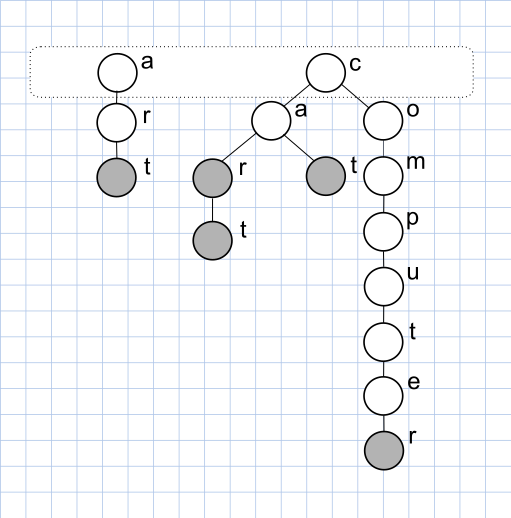
\includegraphics{images/media/02.5-word}
\caption{Crafting root node}\label{fig:5word}
\end{figure}

This operation raises an essential design question: what is the internal
structure of a Trie node? The need to accommodate multiple starting
characters at the root level makes explicit the role of nodes as
branching points rather than mere containers for characters.

\section{Formal definition}\label{formal-definition}

The formal definition of a Trie is based on several fundamental concepts.
First, an alphabet defines the set of symbols that can be used to construct keys.
A key defines an ordered sequence of such symbols, while a node defines the structural elements
used to represent these sequences as paths in the Trie. These concepts are introduced step by step
in the following sections.

\subsection{Alphabet}\label{alphabet}

In the context of this article, an alphabet \(\Sigma\) is a finite, non-empty set of distinct symbols
that can be used to construct Trie keys. A symbol is the smallest indivisible element considered by
the Trie when navigating from one node to another.

Formally,
\begin{equation}
\Sigma = {b_1, b_2, \ldots, b_n}, \qquad |\Sigma| = n > 0.
\end{equation}

The alphabet does not necessarily represent a natural-language alphabet. It defines the set of
possible values that may occur at each position of a key. Consequently, the choice of alphabet depends
on how the indexed data is represented.
The unary case, \(n=1\), is mathematically valid but represents a degenerate Trie in which every node
has at most one outgoing edge. Consequently, the Trie forms a single chain and provides no branching-based
search advantage. The practically relevant cases considered in this article therefore have \(n > 1\).

Table~\ref{tab:alphabetExamples} presents several alphabets relevant to the representations considered in this
and subsequent articles.


\begin{table}[h]
\caption{Examples of alphabets}\label{tab:alphabetExamples}%
\begin{tabular}{@{}l|ll@{}}
\toprule
Example & Set definition & Set cardinality (alphabet power) \\
\midrule
% 1.
Boolean values - binary alphabet &
$\Sigma_{2} = \left\{ 0,1\right\}$ &
$\left| \Sigma_{2} \right| = 2$ \\
% 2.
Small English letters &
\(\Sigma_{26} = \{ a,b,\dots z\}\) &
\(\left| \Sigma_{26} \right| = 26\) \\
% 3.
Unsigned 8-bit integer  &
\(\Sigma_{byte} = \{ 0,1,\dots255\}\) &
\(\left| \Sigma_{byte} \right| = 256\) \\
% 4.
Signed 8-bit integer &
\(\Sigma_{i128} = \{ - 128,\dots127\}\)&
\(\left| \Sigma_{i128} \right| = 128\) \\
\botrule
\end{tabular}
\footnotetext{
}
\end{table}

\noindent

For example, \(\Sigma_{26}\) can represent the 26 lowercase English letters, that was used in previous chapter
during non-formal definition of Trie. While \(\Sigma_{byte}\) can represent
all 256 possible byte values. The latter is particularly relevant for computer-oriented string representations,
including UTF-8, where a string can be processed as a sequence of bytes.

The alphabet used by a Trie therefore defines its branching domain: for every key position, the next symbol must belong
to \(\Sigma\). The size of this alphabet has a direct impact on the memory requirements of node representations, which
becomes particularly important when a node is implemented as a fixed-size lookup table.

\subsection{Key}\label{key}

A key is a finite non-empty sequence of symbols from $\Sigma$:

\begin{equation}
k = b_{1},b_{2} \ldots,
 \mathrm{where}\!:
  b_{i} \in \Sigma  \land  i > 0
\end{equation}

Since this article focuses on the practical use of Tries for database
indexing, a key is not sufficient on its own. Each key must be
associated with a value. Let $V$ denote an arbitrary value domain - such
as integers, floating-point numbers, strings, or, in subsequent
articles, vectors.

A Trie therefore represents a key - value mapping, where a value
\(v = V\) is associated with a key $k$ at its terminal position in the
structure.

\subsection{Node}\label{node}

Throughout this article, a Trie has been described as a tree, which in
turn is a special case of a graph. A graph consists of nodes and edges,
and the following discussion clarifies how these concepts are
interpreted in a Trie designed for practical use in key-value
databases.

The vast majority of modern database indexing structures are based on
B-tree variants, most notably B-trees, B\textsuperscript{+}-trees, and B\textsuperscript{*}-trees \cite{zhang2022memory,idreos2019design}.
      On the one hand, this dominance can be explained by the existence
of mature, well-understood algorithms supporting insertion, deletion,
point queries, and range queries. On the other hand, it is equally
important to consider the influence of modern hardware architectures.

B-tree - based indexes are closely aligned with page-oriented access
patterns, which efficiently exploit hardware mechanisms such as Direct
Memory Access (DMA) and Ultra DMA (UDMA) for transferring large
contiguous blocks of data between storage devices, memory, and
processors \cite{fent2020low,vogel2023towards,lasch2024heterogeneous}. By organizing nodes as disk-sized pages, these
structures minimize I/O operations and achieve high throughput on
external storage.

In contrast, most academic definitions of Tries do not explicitly
address page-organized access. Instead, they typically assume
fine-grained, pointer-based node representations. To bridge this gap, we
begin with a conventional node definition and later extend it to better
exploit page-oriented storage.

\subsubsection{Root Node and Navigation}\label{root-node-and-navigation}

As defined in classical sources \cite{knuthVol3, fds_alg}, a Trie contains a
distinguished root node corresponding to the empty key $\epsilon$. All operations
on the Trie begin at this root.
However, the empty string is not considered a valid key in the
data model used in this work. Consequently, the root does not need to represent
a separate key value. This observation allows the conventional non-functional
root to be replaced by a root node that participates in the same representation as the other
nodes. In particular, the root can contain the payload associated with the first level
of the Trie rather than serving solely as a structural entry point.
The motivation is not merely to eliminate one node. More importantly, treating
the root as an ordinary functional node reduces the number of special cases in subsequent
algorithms. When all nodes follow the same representation and expose the same operations,
algorithms can be expressed at a finer and more uniform granularity: traversal, lookup,
insertion, and node optimization can be defined in terms of a single node abstraction rather than requiring
separate processing for the root. Thus, the distinction between the root and other nodes is not required
by the semantics of the key set, but is primarily a consequence of the conventional representation.
Since the empty string is outside the considered key domain, this distinction can be removed without
changing the set of represented keys.

With the Trie representation established, we can define the lookup operation in terms of a mapping
from a key to either its existence status or its associated value. The simplest form of this
operation is the \textit{Exists} predicate, which determines whether a given key is represented by a terminal
node in the Trie:

\begin{equation}
E(k) \rightarrow \{\mathrm{True},\mathrm{False}\}.
\end{equation}

For the Trie depicted in Figure~\ref{fig:5word}, the predicate evaluates as follows:

\begin{table}[htbp]

\begin{minipage}{\textwidth} % need this to stretch tabular as caption

    \caption{Sample evaluation of Exists (\(E\)) predicate.}\label{tab:queryExists}%
    \begin{tabular}{lp{0.5\linewidth} }
    \toprule
    Query & Result \\
    \midrule
    % 1.
    \(E("art")\) & True \\
    % 2.
    \(E("car")\) & True \\
    % 3.
    \(E("ca")\) & False (no such terminal) \\
    % 4.
    \(E("camp")\) & False \\
    \end{tabular}

\end{minipage}

\end{table}
\noindent


The definition above describes the \textit{result} of a lookup, but does not specify how
this result is obtained. The next question is therefore the computational cost of evaluating $E(k)$.
In particular, the lookup procedure must determine, for each successive symbol of the key, whether
the corresponding outgoing edge exists. The complexity of this operation depends directly on how
the outgoing edges of each Trie node are represented.


\subsubsection{Lookup Complexity with Linear Edge Scanning}
\label{lookup-complexity-with-linear-edge-scanning}

Let us analyze the complexity of the lookup operation \cite{largescalesearch2021} using a naive node representation.
Consider the worst-case scenario in which the requested key does not exist in the Trie, for example, "can".

\begin{enumerate}
  \def\labelenumi{\arabic{enumi}.}
\item Start at the root node.
\item Iterate over all outgoing edges of the root and compare their labels with the first symbol, "c".
 The edge labeled "c" is found.
\item Move to the child corresponding to "c".
Iterate over its outgoing edges and compare their labels with the second symbol, "a". The edge labeled "a" is found.
\item Move to the child corresponding to "a".
Iterate over its outgoing edges and compare their labels with the third symbol, "n" that does not match to any, and
the search terminates with \texttt{False}.
\end{enumerate}


If a node has $N$ outgoing edges, finding a matching edge by linear scanning requires $O(N)$ time.
For a key containing $m$ symbols, the lookup may have to perform such a search at each level of the Trie.
Let $N_i$ denote the number of outgoing edges at the node visited at level $i$. The total lookup complexity is therefore

\begin{equation}
O(N_1 + N_2 + \dots + N_m).
\end{equation}

In the worst case, when each visited node has approximately $N$ outgoing edges, this becomes $O(mN)$.

An obvious improvement is to keep the outgoing edges sorted by their labels. This allows binary search at each node
and reduces the lookup complexity to

\begin{equation}
O(\log N_1 + \dots + \log N_m),
\end{equation}

However, an even more direct approach is to eliminate the need for edge scanning altogether by mapping each
symbol to a predetermined position. This leads to the lookup-table representation described in the following section.

\subsubsection{Lookup Table}
\label{lookup-table}

A common optimization is to provide each node with a lookup table indexed by the alphabet $\Sigma$. In this
representation, as depicted in Figure~\ref{fig:lookupTable}, each possible symbol corresponds to a fixed
slot containing either a reference to a child node or an empty value (\texttt{nil}). So applying lookup table allows:

\begin{itemize}
\item
  to achieve constant-time of child selection,
\item
  to travers directly node symbols \(b_{1},b_{2}\ \dots b_{m}\),
\item
  eliminated search iteration over outgoing edges.
\end{itemize}


\begin{figure}[h]
\centering

\includegraphics[width=0.85\textwidth]{./images/media/03.lookup-table}
\caption{Lookup table example for \(\Sigma_{26}\) alphabet}\label{fig:lookupTable}
\end{figure}


As a result, the complexity of the Exists predicate becomes:

\begin{equation}
O(1 + 1 + \dots + 1) = O(m).
\end{equation}


An additional benefit of this approach is its compatibility with
page-organized access. Fixed-size tables align naturally with cache
lines and memory pages, making this representation more amenable to
high-throughput, hardware-efficient implementations than pointer-heavy,
irregular node layouts.

Another important property of lookup-table based Trie nodes is that
traversal algorithms can rely on a fixed, globally ordered alphabet
within a single page. This guarantees deterministic navigation across
levels of the Trie and enables efficient, branch-free lookup logic.
Later in this article, we will show how this property can be exploited
to improve navigation and traversal performance.

The major drawback of lookup tables, however, is their memory
inefficiency when nodes are sparsely populated. In many cases, a large
fraction of table entries remain unused, yet still consume memory. This
issue becomes particularly visible when indexing natural-language data.

Consider English words over an alphabet \(\Sigma_{26}\). As demonstrated
in prior studies \cite{yau2014distribution, norvig2012english} , English spelling rules forbid most letter
combinations. For example, a word starting with the letter "q" is almost
always followed by "u", creating a strong statistical bias at the second
level of the Trie. As a result, a lookup table allocated for all 26
possible successors at that level will be overwhelmingly empty, leading
to poor space utilization.

Consequently, lookup-table based nodes can be highly inefficient for
sparse or skewed alphabets. This observation motivates the exploration
of alternative representations - most notably hash tables and sorted
arrays - which trade constant-time access for improved space efficiency.
The next section examines these alternatives and analyzes their impact
on lookup performance and memory layout.

\subsubsection{Page Space Optimization}\label{page-space-optimization}

To overcome the space inefficiency of lookup-table - based nodes, we
need to select alternative data structures that satisfy the following
requirements:

\begin{itemize}
\item
  Access complexity better than \(O(N)\) for locating an element
  \(b_{i}\).
\item
  Compatibility with page-based access, favoring linear or contiguous
  memory layouts. (For this reason, linked lists are poor candidates.)
\item
  Support for ordered navigation, which is desirable for prefix scans
  and range-like traversal.
\item
  Space usage significantly smaller than the alphabet size, i.e.:
\begin{equation}
l \ll |\Sigma|.\label{eq:lessThanAlphabet}
\end{equation}

Otherwise, a full lookup table indexed by \(\Sigma\) remains the optimal solution.

\end{itemize}


A widely adopted memory-saving technique is to combine full lookup
tables for densely populated nodes with compact control structures for
sparse nodes. This idea is formalized in the family of data structures
commonly referred to as adaptive Tries or Adaptive Radix Trees
(ART) \cite{leis2013adaptive}.

The core principle is simple: node representations adapt to their
fan-out (population size). When the number of outgoing edges is small,
compact representations are used; as the node becomes denser, the
representation gradually expands. In practice, this expansion is often
performed in powers of two, for example, arrays of size 8, 16, 32, and
so on, until condition (\ref{eq:lessThanAlphabet}) is violated and a full lookup table becomes
justified.

Some approaches \cite{farachcolton2025optimalboundsopenaddressing} propose the use of hash tables with open
addressing for sparse nodes. While effective for lookup, hash tables
lack inherent ordering and introduce additional complexity. Instead, we
can craft a custom node representation that satisfies all previously
stated requirements: fast lookup, ordered navigation, linear memory
layout, and efficient space usage.

We begin with a bitmap that encodes the presence or absence of outgoing
edges. Each bit corresponds to one symbol \(b_{i}\) .

\begin{itemize}
\item
  bit value 1 - means corresponding child exists
\item
  bit value 0 - means no child for that symbol.
\end{itemize}

The bitmap size exactly matches the alphabet size \(|\Sigma|\).
The Exists predicate \(E\left( b_{i} \right)\) is implemented
by a single bit test, yielding constant-time performance. For example,
at Figure~\ref{fig:adaptiveSizedNodes}, symbols "a" and "c" correspond to bits set to 1, while "b"
and "z" correspond to bits set to 0.

\begin{figure}[h]
\centering

\includegraphics{./images/media/04.Adaptive-sized-nodes}
\caption{Combine bitmap with array}\label{fig:adaptiveSizedNodes}
\end{figure}

Modern processors efficiently support bitmap operations using native
integer registers. For an alphabet
\(\left| \Sigma_{byte} \right| = 256\), the bitmap requires only four
64-bit unsigned integers, representing a negligible memory overhead.

To store associated child references or service metadata, the bitmap is
paired with a compact ordered array (Figure ~\ref{fig:bitmapAndArray}). This array stores only
the existing children, eliminating all (\texttt{nil}) entries present in full
lookup tables.

  Key properties of this design:
\begin{itemize}
\item
  The bitmap provides O(1) existence checks.
\item
  The array stores only populated entries.
\item
  Array elements are maintained in sorted order, enabling ordered
  traversal.
\item
  The index into the array is computed using a population count
  (popcount\footnote{
The vast majority of modern CPUs support the POPCNT instruction
 for calculating the rank of a set bit
}) over the bitmap.
\end{itemize}

As a result, this structure removes wasted space while preserving fast
access and ordered navigation.

\begin{figure}[h]
    \centering
    
\includegraphics{./images/media/05.Bitmap-and-Array}
    \caption{Using array of bitmap for lookup}\label{fig:bitmapAndArray}
\end{figure}


Summarizing the properties of this bitmap-array let's articulate:
\begin{itemize}
    \item
      Bitmap operations are directly supported by native CPU instructions.
    \item
      Compact arrays minimize memory footprint while maintaining linear space complexity.
    \item
      Alphabet ordered traversal remains natural and efficient.
    \item Lookup has $O(1)$ complexity for a fixed-size alphabet.
\end{itemize}

yyyyyyyyyyyyyyyyyyyyyyyyyyyyyyyyyyyyy


\section{This is an example for first level head---section head}\label{sec3}

\subsection{This is an example for second level head---subsection head}\label{subsec2}

\subsubsection{This is an example for third level head---subsubsection head}\label{subsubsec2}

Sample body text. Sample body text. Sample body text. Sample body text. Sample body text. Sample body text. Sample body text. Sample body text. 

\section{Equations}\label{sec4}

Equations in \LaTeX\ can either be inline or on-a-line by itself (``display equations''). For
inline equations use the \verb+$...$+ commands. E.g.: The equation
$H\psi = E \psi$ is written via the command \verb+$H \psi = E \psi$+.

For display equations (with auto generated equation numbers)
one can use the equation or align environments:
\begin{equation}
\|\tilde{X}(k)\|^2 \leq\frac{\sum\limits_{i=1}^{p}\left\|\tilde{Y}_i(k)\right\|^2+\sum\limits_{j=1}^{q}\left\|\tilde{Z}_j(k)\right\|^2 }{p+q}.\label{eq1}
\end{equation}
where,
\begin{align}
D_\mu &=  \partial_\mu - ig \frac{\lambda^a}{2} A^a_\mu \nonumber \\
F^a_{\mu\nu} &= \partial_\mu A^a_\nu - \partial_\nu A^a_\mu + g f^{abc} A^b_\mu A^a_\nu \label{eq2}
\end{align}
Notice the use of \verb+\nonumber+ in the align environment at the end
of each line, except the last, so as not to produce equation numbers on
lines where no equation numbers are required. The \verb+\label{}+ command
should only be used at the last line of an align environment where
\verb+\nonumber+ is not used.
\begin{equation}
Y_\infty = \left( \frac{m}{\textrm{GeV}} \right)^{-3}
    \left[ 1 + \frac{3 \ln(m/\textrm{GeV})}{15}
    + \frac{\ln(c_2/5)}{15} \right]
\end{equation}
The class file also supports the use of \verb+\mathbb{}+, \verb+\mathscr{}+ and
\verb+\mathcal{}+ commands. As such \verb+\mathbb{R}+, \verb+\mathscr{R}+
and \verb+\mathcal{R}+ produces $\mathbb{R}$, $\mathscr{R}$ and $\mathcal{R}$
respectively (refer Subsubsection~\ref{subsubsec2}).

\section{Tables}\label{sec5}

Tables can be inserted via the normal table and tabular environment. To put
footnotes inside tables you should use \verb+\footnotetext[]{...}+ tag.
The footnote appears just below the table itself (refer Tables~\ref{tab1} and \ref{tab2}). 
For the corresponding footnotemark use \verb+\footnotemark[...]+

\begin{table}[h]
\caption{Caption text}\label{tab1}%
\begin{tabular}{@{}llll@{}}
\toprule
Column 1 & Column 2  & Column 3 & Column 4\\
\midrule
row 1    & data 1   & data 2  & data 3  \\
row 2    & data 4   & data 5\footnotemark[1]  & data 6  \\
row 3    & data 7   & data 8  & data 9\footnotemark[2]  \\
\botrule
\end{tabular}
\footnotetext{Source: This is an example of table footnote. This is an example of table footnote.}
\footnotetext[1]{Example for a first table footnote. This is an example of table footnote.}
\footnotetext[2]{Example for a second table footnote. This is an example of table footnote.}
\end{table}

\noindent
The input format for the above table is as follows:

%%=============================================%%
%% For presentation purpose, we have included  %%
%% \bigskip command. Please ignore this.       %%
%%=============================================%%
\bigskip
\begin{verbatim}
\begin{table}[<placement-specifier>]
\caption{<table-caption>}\label{<table-label>}%
\begin{tabular}{@{}llll@{}}
\toprule
Column 1 & Column 2 & Column 3 & Column 4\\
\midrule
row 1 & data 1 & data 2	 & data 3 \\
row 2 & data 4 & data 5\footnotemark[1] & data 6 \\
row 3 & data 7 & data 8	 & data 9\footnotemark[2]\\
\botrule
\end{tabular}
\footnotetext{Source: This is an example of table footnote. 
This is an example of table footnote.}
\footnotetext[1]{Example for a first table footnote.
This is an example of table footnote.}
\footnotetext[2]{Example for a second table footnote. 
This is an example of table footnote.}
\end{table}
\end{verbatim}
\bigskip
%%=============================================%%
%% For presentation purpose, we have included  %%
%% \bigskip command. Please ignore this.       %%
%%=============================================%%

\begin{table}[h]
\caption{Example of a lengthy table which is set to full textwidth}\label{tab2}
\begin{tabular*}{\textwidth}{@{\extracolsep\fill}lcccccc}
\toprule%
& \multicolumn{3}{@{}c@{}}{Element 1\footnotemark[1]} & \multicolumn{3}{@{}c@{}}{Element 2\footnotemark[2]} \\\cmidrule{2-4}\cmidrule{5-7}%
Project & Energy & $\sigma_{calc}$ & $\sigma_{expt}$ & Energy & $\sigma_{calc}$ & $\sigma_{expt}$ \\
\midrule
Element 3  & 990 A & 1168 & $1547\pm12$ & 780 A & 1166 & $1239\pm100$\\
Element 4  & 500 A & 961  & $922\pm10$  & 900 A & 1268 & $1092\pm40$\\
\botrule
\end{tabular*}
\footnotetext{Note: This is an example of table footnote. This is an example of table footnote this is an example of table footnote this is an example of~table footnote this is an example of table footnote.}
\footnotetext[1]{Example for a first table footnote.}
\footnotetext[2]{Example for a second table footnote.}
\end{table}

In case of double column layout, tables which do not fit in single column width should be set to full text width. For this, you need to use \verb+\begin{table*}+ \verb+...+ \verb+\end{table*}+ instead of \verb+\begin{table}+ \verb+...+ \verb+\end{table}+ environment. Lengthy tables which do not fit in textwidth should be set as rotated table. For this, you need to use \verb+\begin{sidewaystable}+ \verb+...+ \verb+\end{sidewaystable}+ instead of \verb+\begin{table*}+ \verb+...+ \verb+\end{table*}+ environment. This environment puts tables rotated to single column width. For tables rotated to double column width, use \verb+\begin{sidewaystable*}+ \verb+...+ \verb+\end{sidewaystable*}+.

\begin{sidewaystable}
\caption{Tables which are too long to fit, should be written using the ``sidewaystable'' environment as shown here}\label{tab3}
\begin{tabular*}{\textheight}{@{\extracolsep\fill}lcccccc}
\toprule%
& \multicolumn{3}{@{}c@{}}{Element 1\footnotemark[1]}& \multicolumn{3}{@{}c@{}}{Element\footnotemark[2]} \\\cmidrule{2-4}\cmidrule{5-7}%
Projectile & Energy	& $\sigma_{calc}$ & $\sigma_{expt}$ & Energy & $\sigma_{calc}$ & $\sigma_{expt}$ \\
\midrule
Element 3 & 990 A & 1168 & $1547\pm12$ & 780 A & 1166 & $1239\pm100$ \\
Element 4 & 500 A & 961  & $922\pm10$  & 900 A & 1268 & $1092\pm40$ \\
Element 5 & 990 A & 1168 & $1547\pm12$ & 780 A & 1166 & $1239\pm100$ \\
Element 6 & 500 A & 961  & $922\pm10$  & 900 A & 1268 & $1092\pm40$ \\
\botrule
\end{tabular*}
\footnotetext{Note: This is an example of table footnote this is an example of table footnote this is an example of table footnote this is an example of~table footnote this is an example of table footnote.}
\footnotetext[1]{This is an example of table footnote.}
\end{sidewaystable}

\section{Figures}\label{sec6}

As per the \LaTeX\ standards you need to use eps images for \LaTeX\ compilation and \verb+pdf/jpg/png+ images for \verb+PDFLaTeX+ compilation. This is one of the major difference between \LaTeX\ and \verb+PDFLaTeX+. Each image should be from a single input .eps/vector image file. Avoid using subfigures. The command for inserting images for \LaTeX\ and \verb+PDFLaTeX+ can be generalized. The package used to insert images in \verb+LaTeX/PDFLaTeX+ is the graphicx package. Figures can be inserted via the normal figure environment as shown in the below example:

%%=============================================%%
%% For presentation purpose, we have included  %%
%% \bigskip command. Please ignore this.       %%
%%=============================================%%
\bigskip
\begin{verbatim}
\begin{figure}[<placement-specifier>]
\centering
\includegraphics{<eps-file>}
\caption{<figure-caption>}\label{<figure-label>}
\end{figure}
\end{verbatim}
\bigskip
%%=============================================%%
%% For presentation purpose, we have included  %%
%% \bigskip command. Please ignore this.       %%
%%=============================================%%

\begin{figure}[h]
\centering
\includegraphics[width=0.9\textwidth]{images/media/image1}
\caption{This is a widefig. This is an example of long caption this is an example of long caption  this is an example of long caption this is an example of long caption}\label{fig1}
\end{figure}

In case of double column layout, the above format puts figure captions/images to single column width. To get spanned images, we need to provide \verb+\begin{figure*}+ \verb+...+ \verb+\end{figure*}+.

For sample purpose, we have included the width of images in the optional argument of \verb+\includegraphics+ tag. Please ignore this. 

\section{Algorithms, Program codes and Listings}\label{sec7}

Packages \verb+algorithm+, \verb+algorithmicx+ and \verb+algpseudocode+ are used for setting algorithms in \LaTeX\ using the format:

%%=============================================%%
%% For presentation purpose, we have included  %%
%% \bigskip command. Please ignore this.       %%
%%=============================================%%
\bigskip
\begin{verbatim}
\begin{algorithm}
\caption{<alg-caption>}\label{<alg-label>}
\begin{algorithmic}[1]
. . .
\end{algorithmic}
\end{algorithm}
\end{verbatim}
\bigskip
%%=============================================%%
%% For presentation purpose, we have included  %%
%% \bigskip command. Please ignore this.       %%
%%=============================================%%

You may refer above listed package documentations for more details before setting \verb+algorithm+ environment. For program codes, the ``verbatim'' package is required and the command to be used is \verb+\begin{verbatim}+ \verb+...+ \verb+\end{verbatim}+. 

Similarly, for \verb+listings+, use the \verb+listings+ package. \verb+\begin{lstlisting}+ \verb+...+ \verb+\end{lstlisting}+ is used to set environments similar to \verb+verbatim+ environment. Refer to the \verb+lstlisting+ package documentation for more details.

A fast exponentiation procedure:

\lstset{texcl=true,basicstyle=\small\sf,commentstyle=\small\rm,mathescape=true,escapeinside={(*}{*)}}
\begin{lstlisting}
begin
  for $i:=1$ to $10$ step $1$ do
      expt($2,i$);  
      newline() od                (*\textrm{Comments will be set flush to the right margin}*)
where
proc expt($x,n$) $\equiv$
  $z:=1$;
  do if $n=0$ then exit fi;
     do if odd($n$) then exit fi;                 
        comment: (*\textrm{This is a comment statement;}*)
        $n:=n/2$; $x:=x*x$ od;
     { $n>0$ };
     $n:=n-1$; $z:=z*x$ od;
  print($z$). 
end
\end{lstlisting}

\begin{algorithm}
\caption{Calculate $y = x^n$}\label{algo1}
\begin{algorithmic}[1]
\Require $n \geq 0 \vee x \neq 0$
\Ensure $y = x^n$ 
\State $y \Leftarrow 1$
\If{$n < 0$}\label{algln2}
        \State $X \Leftarrow 1 / x$
        \State $N \Leftarrow -n$
\Else
        \State $X \Leftarrow x$
        \State $N \Leftarrow n$
\EndIf
\While{$N \neq 0$}
        \If{$N$ is even}
            \State $X \Leftarrow X \times X$
            \State $N \Leftarrow N / 2$
        \Else[$N$ is odd]
            \State $y \Leftarrow y \times X$
            \State $N \Leftarrow N - 1$
        \EndIf
\EndWhile
\end{algorithmic}
\end{algorithm}

%%=============================================%%
%% For presentation purpose, we have included  %%
%% \bigskip command. Please ignore this.       %%
%%=============================================%%
\bigskip
\begin{minipage}{\hsize}%
\lstset{frame=single,framexleftmargin=-1pt,framexrightmargin=-17pt,framesep=12pt,linewidth=0.98\textwidth,language=pascal}% Set your language (you can change the language for each code-block optionally)
%%% Start your code-block
\begin{lstlisting}
for i:=maxint to 0 do
begin
{ do nothing }
end;
Write('Case insensitive ');
Write('Pascal keywords.');
\end{lstlisting}
\end{minipage}

\section{Cross referencing}\label{sec8}

Environments such as figure, table, equation and align can have a label
declared via the \verb+\label{#label}+ command. For figures and table
environments use the \verb+\label{}+ command inside or just
below the \verb+\caption{}+ command. You can then use the
\verb+\ref{#label}+ command to cross-reference them. As an example, consider
the label declared for Figure~\ref{fig1} which is
\verb+\label{fig1}+. To cross-reference it, use the command 
\verb+Figure \ref{fig1}+, for which it comes up as
``Figure~\ref{fig1}''. 

To reference line numbers in an algorithm, consider the label declared for the line number 2 of Algorithm~\ref{algo1} is \verb+\label{algln2}+. To cross-reference it, use the command \verb+\ref{algln2}+ for which it comes up as line~\ref{algln2} of Algorithm~\ref{algo1}.

\subsection{Details on reference citations}\label{subsec7}

Standard \LaTeX\ permits only numerical citations. To support both numerical and author-year citations this template uses \verb+natbib+ \LaTeX\ package. For style guidance please refer to the template user manual.

Here is an example for \verb+\cite{...}+: \cite{bib1}. Another example for \verb+\citep{...}+: \citep{bib2}. For author-year citation mode, \verb+\cite{...}+ prints Jones et al. (1990) and \verb+\citep{...}+ prints (Jones et al., 1990).

All cited bib entries are printed at the end of this article: \cite{bib3}, \cite{bib4}, \cite{bib5}, \cite{bib6}, \cite{bib7}, \cite{bib8}, \cite{bib9}, \cite{bib10}, \cite{bib11}, \cite{bib12} and \cite{bib13}.

\section{Examples for theorem like environments}\label{sec10}

For theorem like environments, we require \verb+amsthm+ package. There are three types of predefined theorem styles exists---\verb+thmstyleone+, \verb+thmstyletwo+ and \verb+thmstylethree+ 

%%=============================================%%
%% For presentation purpose, we have included  %%
%% \bigskip command. Please ignore this.       %%
%%=============================================%%
\bigskip
\begin{tabular}{|l|p{19pc}|}
\hline
\verb+thmstyleone+ & Numbered, theorem head in bold font and theorem text in italic style \\\hline
\verb+thmstyletwo+ & Numbered, theorem head in roman font and theorem text in italic style \\\hline
\verb+thmstylethree+ & Numbered, theorem head in bold font and theorem text in roman style \\\hline
\end{tabular}
\bigskip
%%=============================================%%
%% For presentation purpose, we have included  %%
%% \bigskip command. Please ignore this.       %%
%%=============================================%%

For mathematics journals, theorem styles can be included as shown in the following examples:

\begin{theorem}[Theorem subhead]\label{thm1}
Example theorem text. Example theorem text. Example theorem text. Example theorem text. Example theorem text. 
Example theorem text. Example theorem text. Example theorem text. Example theorem text. Example theorem text. 
Example theorem text. 
\end{theorem}

Sample body text. Sample body text. Sample body text. Sample body text. Sample body text. Sample body text. Sample body text. Sample body text.

\begin{proposition}
Example proposition text. Example proposition text. Example proposition text. Example proposition text. Example proposition text. 
Example proposition text. Example proposition text. Example proposition text. Example proposition text. Example proposition text. 
\end{proposition}

Sample body text. Sample body text. Sample body text. Sample body text. Sample body text. Sample body text. Sample body text. Sample body text.

\begin{example}
Phasellus adipiscing semper elit. Proin fermentum massa
ac quam. Sed diam turpis, molestie vitae, placerat a, molestie nec, leo. Maecenas lacinia. Nam ipsum ligula, eleifend
at, accumsan nec, suscipit a, ipsum. Morbi blandit ligula feugiat magna. Nunc eleifend consequat lorem. 
\end{example}

Sample body text. Sample body text. Sample body text. Sample body text. Sample body text. Sample body text. Sample body text. Sample body text.

\begin{remark}
Phasellus adipiscing semper elit. Proin fermentum massa
ac quam. Sed diam turpis, molestie vitae, placerat a, molestie nec, leo. Maecenas lacinia. Nam ipsum ligula, eleifend
at, accumsan nec, suscipit a, ipsum. Morbi blandit ligula feugiat magna. Nunc eleifend consequat lorem. 
\end{remark}

Sample body text. Sample body text. Sample body text. Sample body text. Sample body text. Sample body text. Sample body text. Sample body text.

\begin{definition}[Definition sub head]
Example definition text. Example definition text. Example definition text. Example definition text. Example definition text. Example definition text. Example definition text. Example definition text. 
\end{definition}

Additionally a predefined ``proof'' environment is available: \verb+\begin{proof}+ \verb+...+ \verb+\end{proof}+. This prints a ``Proof'' head in italic font style and the ``body text'' in roman font style with an open square at the end of each proof environment. 

\begin{proof}
Example for proof text. Example for proof text. Example for proof text. Example for proof text. Example for proof text. Example for proof text. Example for proof text. Example for proof text. Example for proof text. Example for proof text. 
\end{proof}

Sample body text. Sample body text. Sample body text. Sample body text. Sample body text. Sample body text. Sample body text. Sample body text.

\begin{proof}[Proof of Theorem~{\upshape\ref{thm1}}]
Example for proof text. Example for proof text. Example for proof text. Example for proof text. Example for proof text. Example for proof text. Example for proof text. Example for proof text. Example for proof text. Example for proof text. 
\end{proof}

\noindent
For a quote environment, use \verb+\begin{quote}...\end{quote}+
\begin{quote}
Quoted text example. Aliquam porttitor quam a lacus. Praesent vel arcu ut tortor cursus volutpat. In vitae pede quis diam bibendum placerat. Fusce elementum
convallis neque. Sed dolor orci, scelerisque ac, dapibus nec, ultricies ut, mi. Duis nec dui quis leo sagittis commodo.
\end{quote}

Sample body text. Sample body text. Sample body text. Sample body text. Sample body text (refer Figure~\ref{fig1}). Sample body text. Sample body text. Sample body text (refer Table~\ref{tab3}). 

\section{Methods}\label{sec11}

Topical subheadings are allowed. Authors must ensure that their Methods section includes adequate experimental and characterization data necessary for others in the field to reproduce their work. Authors are encouraged to include RIIDs where appropriate. 

\textbf{Ethical approval declarations} (only required where applicable) Any article reporting experiment/s carried out on (i)~live vertebrate (or higher invertebrates), (ii)~humans or (iii)~human samples must include an unambiguous statement within the methods section that meets the following requirements: 

\begin{enumerate}[1.]
\item Approval: a statement which confirms that all experimental protocols were approved by a named institutional and/or licensing committee. Please identify the approving body in the methods section

\item Accordance: a statement explicitly saying that the methods were carried out in accordance with the relevant guidelines and regulations

\item Informed consent (for experiments involving humans or human tissue samples): include a statement confirming that informed consent was obtained from all participants and/or their legal guardian/s
\end{enumerate}

If your manuscript includes potentially identifying patient/participant information, or if it describes human transplantation research, or if it reports results of a clinical trial then  additional information will be required. Please visit (\url{https://www.nature.com/nature-research/editorial-policies}) for Nature Portfolio journals, (\url{https://www.springer.com/gp/authors-editors/journal-author/journal-author-helpdesk/publishing-ethics/14214}) for Springer Nature journals, or (\url{https://www.biomedcentral.com/getpublished/editorial-policies\#ethics+and+consent}) for BMC.

\section{Discussion}\label{sec12}

Discussions should be brief and focused. In some disciplines use of Discussion or `Conclusion' is interchangeable. It is not mandatory to use both. Some journals prefer a section `Results and Discussion' followed by a section `Conclusion'. Please refer to Journal-level guidance for any specific requirements. 

\section{Conclusion}\label{sec13}

Conclusions may be used to restate your hypothesis or research question, restate your major findings, explain the relevance and the added value of your work, highlight any limitations of your study, describe future directions for research and recommendations. 

In some disciplines use of Discussion or 'Conclusion' is interchangeable. It is not mandatory to use both. Please refer to Journal-level guidance for any specific requirements. 

\backmatter

\bmhead{Supplementary information}

If your article has accompanying supplementary file/s please state so here. 

Authors reporting data from electrophoretic gels and blots should supply the full unprocessed scans for key as part of their Supplementary information. This may be requested by the editorial team/s if it is missing.

Please refer to Journal-level guidance for any specific requirements.

\bmhead{Acknowledgements}

Acknowledgements are not compulsory. Where included they should be brief. Grant or contribution numbers may be acknowledged.

Please refer to Journal-level guidance for any specific requirements.

\section*{Declarations}

Some journals require declarations to be submitted in a standardised format. Please check the Instructions for Authors of the journal to which you are submitting to see if you need to complete this section. If yes, your manuscript must contain the following sections under the heading `Declarations':

\begin{itemize}
\item Funding
\item Conflict of interest/Competing interests (check journal-specific guidelines for which heading to use)
\item Ethics approval and consent to participate
\item Consent for publication
\item Data availability 
\item Materials availability
\item Code availability 
\item Author contribution
\end{itemize}

\noindent
If any of the sections are not relevant to your manuscript, please include the heading and write `Not applicable' for that section. 

%%===================================================%%
%% For presentation purpose, we have included        %%
%% \bigskip command. Please ignore this.             %%
%%===================================================%%
\bigskip
\begin{flushleft}%
Editorial Policies for:

\bigskip\noindent
Springer journals and proceedings: \url{https://www.springer.com/gp/editorial-policies}

\bigskip\noindent
Nature Portfolio journals: \url{https://www.nature.com/nature-research/editorial-policies}

\bigskip\noindent
\textit{Scientific Reports}: \url{https://www.nature.com/srep/journal-policies/editorial-policies}

\bigskip\noindent
BMC journals: \url{https://www.biomedcentral.com/getpublished/editorial-policies}
\end{flushleft}

\begin{appendices}

\section{Section title of first appendix}\label{secA1}

An appendix contains supplementary information that is not an essential part of the text itself but which may be helpful in providing a more comprehensive understanding of the research problem or it is information that is too cumbersome to be included in the body of the paper.

%%=============================================%%
%% For submissions to Nature Portfolio Journals %%
%% please use the heading ``Extended Data''.   %%
%%=============================================%%

%%=============================================================%%
%% Sample for another appendix section			       %%
%%=============================================================%%

%% \section{Example of another appendix section}\label{secA2}%
%% Appendices may be used for helpful, supporting or essential material that would otherwise 
%% clutter, break up or be distracting to the text. Appendices can consist of sections, figures, 
%% tables and equations etc.

\end{appendices}

%%===========================================================================================%%
%% If you are submitting to one of the Nature Portfolio journals, using the eJP submission   %%
%% system, please include the references within the manuscript file itself. You may do this  %%
%% by copying the reference list from your .bbl file, paste it into the main manuscript .tex %%
%% file, and delete the associated \verb+\bibliography+ commands.                            %%
%%===========================================================================================%%

\bibliography{sn-bibliography}% common bib file
%% if required, the content of .bbl file can be included here once bbl is generated
%%\input sn-article.bbl

\end{document}
